\begin{figure*}
\begin{subfigure}[b]{0.46\textwidth}
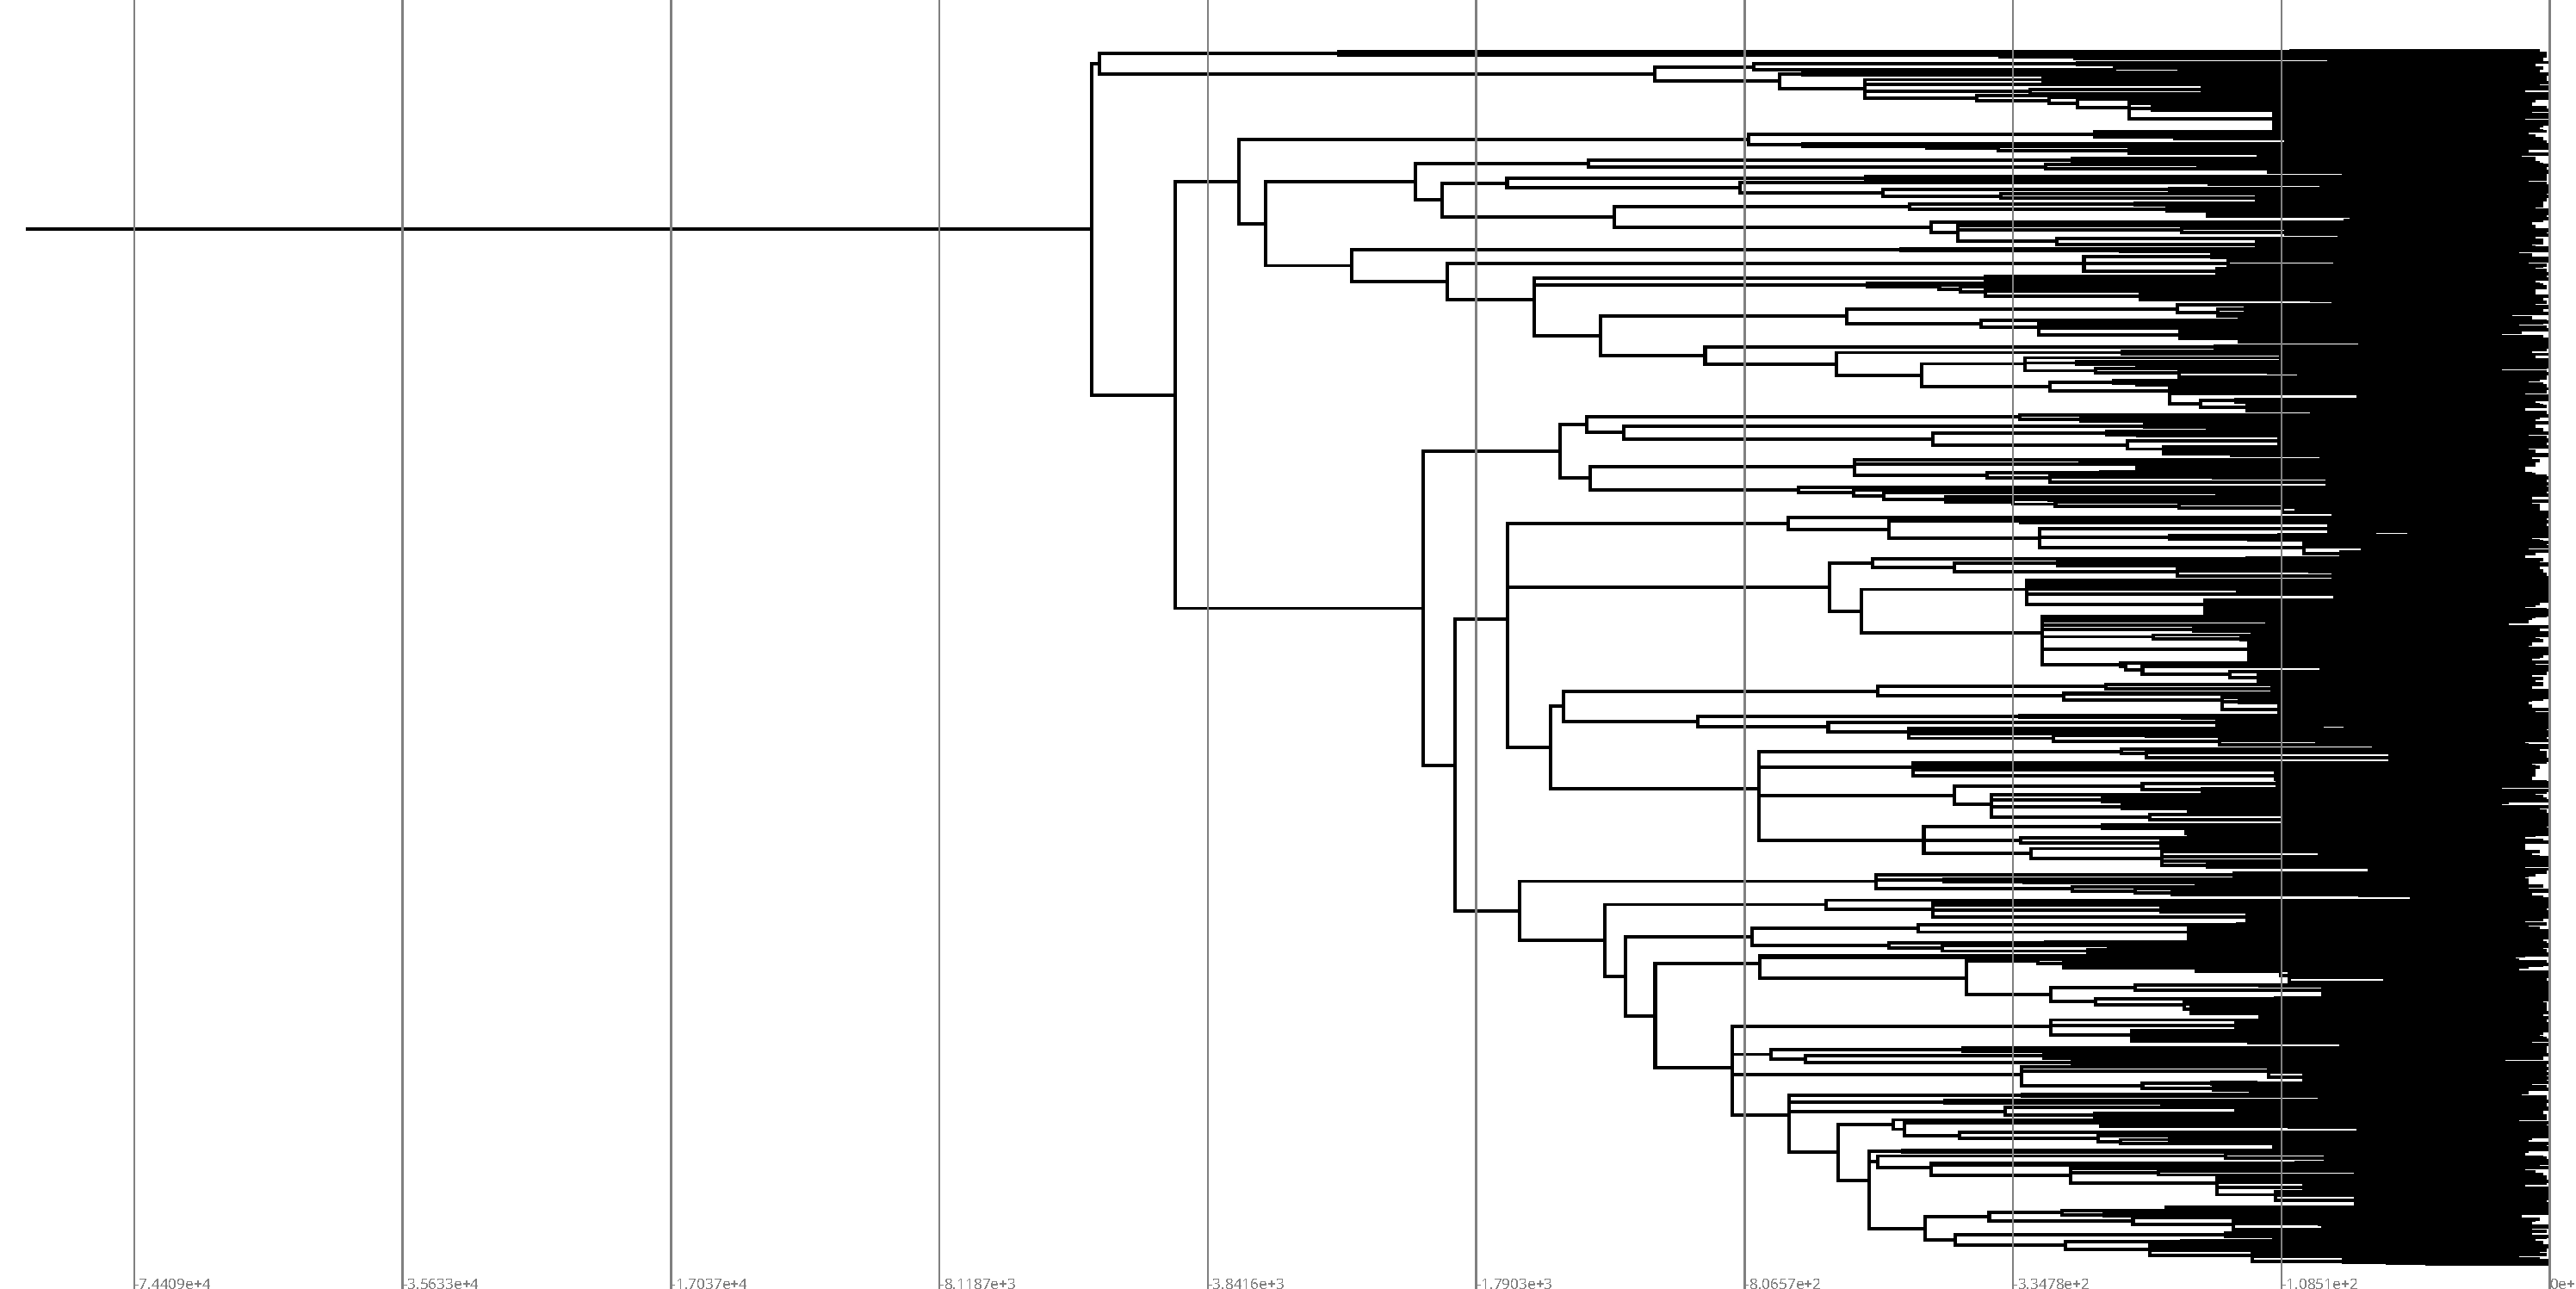
\includegraphics[height=0.12\textheight,width=\textwidth]{img/perfect-tree-phylogenies-log/avida-genome/model=avida+taxon=genome+treatment=plain+seed=1+phylogeny-snapshot-100000.pdf}
    % \end{noindent}
    \caption{%
      genome-level tracking}
    % \label{fig:perfect-tree-phylogenies-log:TODO}
  \end{subfigure}
  \hfill
  \begin{subfigure}[b]{0.46\textwidth}
    % \begin{noindent}
    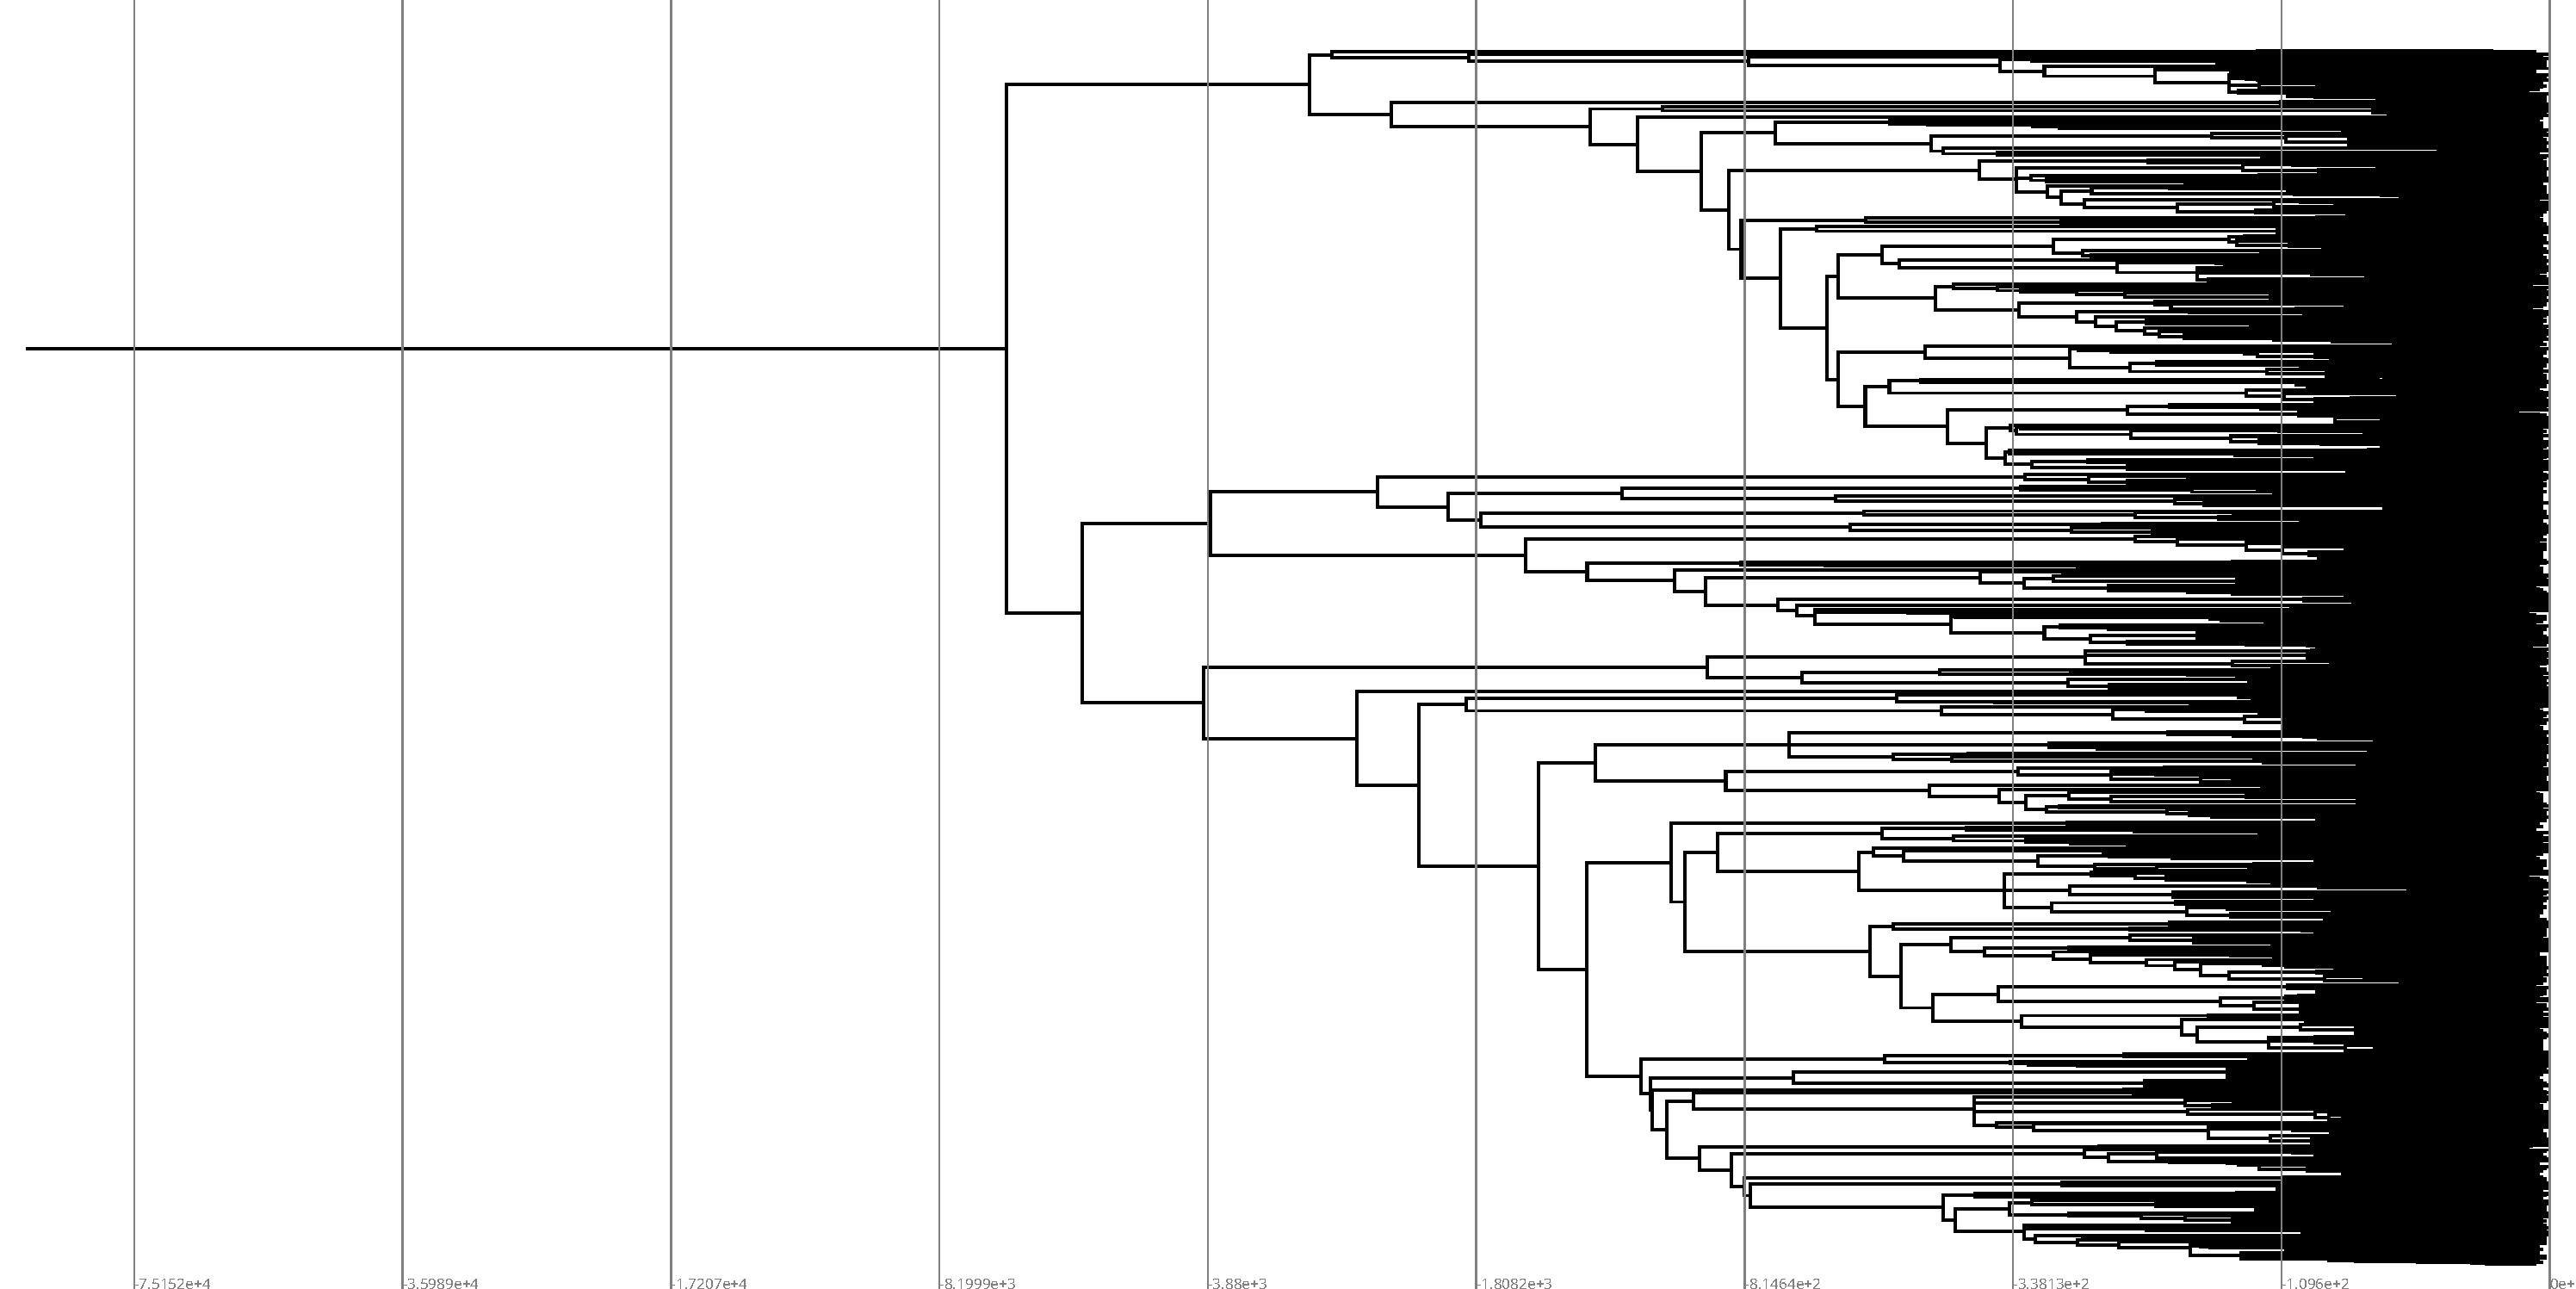
\includegraphics[height=0.12\textheight,width=\textwidth]{img/perfect-tree-phylogenies-log/avida-organism/model=avida+taxon=organism+treatment=plain_individual+seed=1+phylogeny-snapshot-100000.pdf}
    % \end{noindent}
    \caption{%
      organism-level tracking}
    % \label{fig:perfect-tree-phylogenies-log:TODO}
  \end{subfigure}
  \caption{%
    \textbf{Sample reference phylogenies from Avida under ``plain'' regime.}
    Time axis is log-scale.
  }
  \label{fig:perfect-tree-phylogenies-log-avida}
\end{figure*}
